% Created 2020-09-29 Tue 22:59
% Intended LaTeX compiler: lualatex
\documentclass[11pt]{article}
\usepackage{graphicx}
\usepackage{grffile}
\usepackage{longtable}
\usepackage{wrapfig}
\usepackage{rotating}
\usepackage[normalem]{ulem}
\usepackage{amsmath}
\usepackage{textcomp}
\usepackage{amssymb}
\usepackage{capt-of}
\usepackage{hyperref}
\usepackage{tabularx}
\usepackage{etoolbox}
\makeatletter
\def\dontdofcolorbox{\renewcommand\fcolorbox[4][]{##4}}
\AtBeginEnvironment{minted}{\dontdofcolorbox}
\makeatother
\usepackage[newfloat]{minted}
\usepackage{unicode-math}
\usepackage{unicode}
\usepackage{pdfpages}
\author{Mark Armstrong}
\date{\today}
\title{Trees in Prolog}
\hypersetup{
   pdfauthor={Mark Armstrong},
   pdftitle={Trees in Prolog},
   pdfkeywords={},
   pdfsubject={A demonstration of how to represent tree-like data in Prolog.},
   pdfcreator={Emacs 27.0.90 (Org mode 9.4)},
   pdflang={English},
   colorlinks,
   linkcolor=blue,
   citecolor=blue,
   urlcolor=blue
   }
\begin{document}

\maketitle
\tableofcontents


\section{Introduction}
\label{sec:org447d69c}
These notes were created for, and in some parts \textbf{during},
the lecture on September 25th and the following tutorials.

\section{Motivation}
\label{sec:org14ea66b}
So far in this course,
\begin{itemize}
\item we have had a homework on defining different tree datatypes
in Scala, and
\item we have discussed in lectures how trees are used
as the internal and formal representation of programs.
\end{itemize}

Now, in keeping with this theme, let us discuss
how we can reason about trees in Prolog.
This information will be necessary for the sort of programs
we wish to write later on.

\section{Datatypes in Prolog}
\label{sec:org0f7b8e5}
We have previously discussed that there are
four classes of Prolog terms;
\begin{itemize}
\item \emph{numbers},
\begin{itemize}
\item (including both integers and floats)
\end{itemize}
\item \emph{atoms}, which include
words beginning with lower case letters
and strings in single quotes,
\item \emph{variables}, which begin with upper case letters, and
\item \emph{compound terms}
\begin{itemize}
\item (which consist of a \emph{functor} atom and a number
of \emph{arguments} applied to that functor,
\item such as \texttt{isPrime(5)}.)
\end{itemize}
\end{itemize}

These are, in fact, the basic types defined in the Prolog standard.
\begin{itemize}
\item See the \href{https://www.swi-prolog.org/datatypes.html}{SWI Prolog documentation}.
\item There is some hierarchy among the types
(see the next section.)
\item Other types, or even the ability for user-defined types,
may be added as extensions. But in basic Prolog, there are only
the above.
\end{itemize}

Of course, we use in SWI Prolog the list type it provides as well.
But for this course, that is the only extension we will use.
So we must find a way to represent trees with the above.

\section{Aside: the type hierarchy in Prolog}
\label{sec:orgae04564}
In the above linked SWI Prolog documentation on types,
\href{https://github.com/dtonhofer}{David Tonhofer} in the comments links to his
\href{https://github.com/dtonhofer/prolog\_notes/blob/master/swipl\_notes/about\_swipl\_data\_types/swipl\_data\_type\_tree/swipl\_data\_type\_tree.pdf}{Prolog type chart}
and \href{https://github.com/dtonhofer/prolog\_notes/tree/master/swipl\_notes/about\_swipl\_data\_types}{notes}
on the subject of SWI Prolog types.

We include that type chart here for your interest.
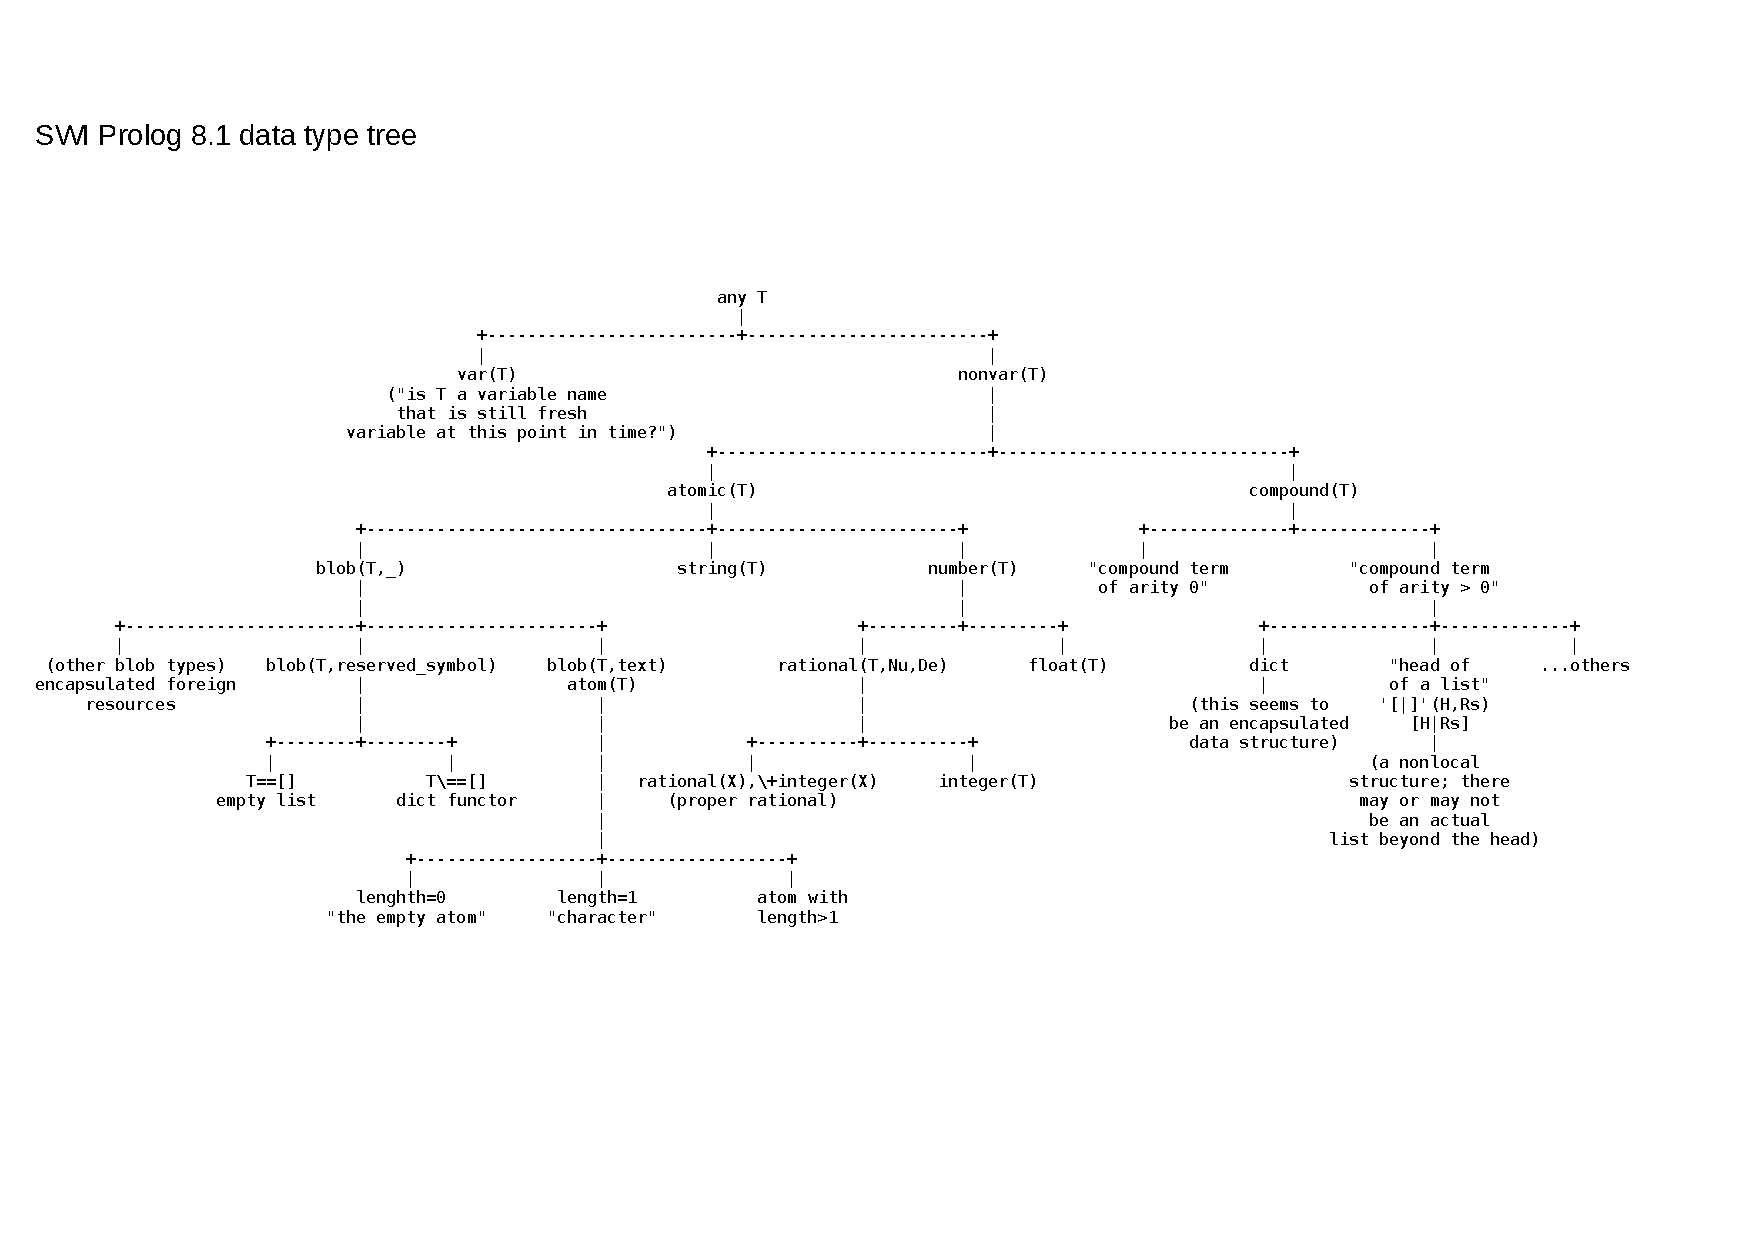
\includepdf[pages=-,width=\pagewidth]{./media/swipl_data_type_tree.pdf}

The \href{https://raw.githubusercontent.com/dtonhofer/prolog\_notes/1057c149ebc145d1df38cc5d1b82b1eaefe925c3/swipl\_notes/about\_swipl\_data\_types/swipl\_data\_type\_tree/swipl\_data\_type\_tree.svg}{detailed SVG} can be quite interesting to examine;
it is far too dense to fit on this page, though.

\section{Tuples}
\label{sec:org495266c}
From Pierce's “\href{https://ebookcentral.proquest.com/lib/mcmu/detail.action?docID=3338823}{Types and Programming Languages}”,
(chapter 11, “Simple Extensions”)
\begin{quote}
Most programming languages provide a variety of ways
of building compound data structures.
The simplest of these is pairs,
or more generally tuples, of values.
\end{quote}

For instance, in Haskell-like notation, the following are tuples.
\begin{minted}[breaklines=true]{text}
(1,2,3) : (Int, Int, Int)
("hello", 1) : (String, Int)
("hello") : (String)
() : ()
\end{minted}

Tuple types differ from lists in that
\begin{itemize}
\item tuples are always heterogeneous,
whereas lists are often homogeneous
\begin{itemize}
\item (that is, tuples can contain a mixture of types), and
\end{itemize}
\item tuples have a fixed length (built into the type).
\end{itemize}

A Prolog compound term of the form \texttt{label(a1,…,an)} can be viewed
as an \texttt{n}-ary tuple along with the label \texttt{label},
and we will use this fact to construct trees in Prolog.

\section{Trees as tuples}
\label{sec:org5270c03}
\subsection{The original tree types}
\label{sec:orgcbfeb4a}
Recall the types \texttt{BinTree} and \texttt{LeafTree} from homework 1.
\begin{minted}[breaklines=true]{scala}
sealed trait LeafTree[A]
case class Leaf[A](a: A) extends LeafTree[A]
case class Branch[A](l: LeafTree[A], r: LeafTree[A]) extends LeafTree[A]

sealed trait BinTree[A]
case class Empty[A]() extends BinTree[A]
case class Node[A](l: BinTree[A], a: A, r: BinTree[A]) extends BinTree[A]
\end{minted}
or in briefer Haskell syntax,
\begin{minted}[breaklines=true]{haskell}
data LeafTree a = Leaf a | Branch (LeafTree a) (LeafTree a)
data BinTree a = Empty | Node (BinTree a) a (BinTree a)
\end{minted}
(for the remainder of the course, if we discuss these types,
we will assume constructors of this shape.)

\subsection{Tupling the arguments}
\label{sec:orgfcb0bd0}
Consider the parameters of each constructor.
\begin{itemize}
\item \texttt{Leaf} has a single parameter of type \texttt{A}.
\item \texttt{Branch} has two parameters of type \texttt{LeafTree A}.
\item \texttt{Empty} does have a parameter, of type \texttt{Unit}.
\begin{itemize}
\item The only value of type \texttt{Unit} being \texttt{()}.
\end{itemize}
\item \texttt{Node} has three parameters of types \texttt{BinTree A}, \texttt{A}, and \texttt{BinTree A}.
\end{itemize}

We could isomorphically define constructors
which each took a single \emph{tuple} as parameter.
\begin{itemize}
\item \texttt{Leaf′} would have a parameter of type \texttt{Tuple1[A]}.
\begin{itemize}
\item To construct a singleton tuple with value \texttt{v}, use \texttt{Tuple1(v)}.
\item For instance, \texttt{Tuple1(5) : Tuple1[Int]}.
\end{itemize}
\item \texttt{Branch′} would have a parameter of type \texttt{Tuple2[LeafTree A, LeafTree A]}.
\item \texttt{Empty′} is the same as \texttt{Empty}, taking a parameter of type \texttt{Unit}.
\begin{itemize}
\item There is no \texttt{Tuple0} type in Scala, but \texttt{Unit} is isomorphic.
\end{itemize}
\item \texttt{Node′} would have a parameter of type \texttt{Tuple3[BinTree A, A, BinTree A]}.
\end{itemize}
We have to say \emph{isomorphically} rather than \emph{equivalently} because
these constructors as \textbf{not} equivalent to the previous versions
(except for \texttt{Empty′}.) But they are \emph{isomorphic}, because they can represent
the same trees, and we have a 1-1 correspondence between them.

The Haskell naming of the tuple type would make
these descriptions briefer.
\begin{itemize}
\item \texttt{Leaf′} would have a parameter of type \texttt{(A)}.
\item \texttt{Branch′} would have a parameter of type \texttt{(LeafTree A, LeafTree A)}.
\item \texttt{Empty′} would have a parameter of type \texttt{()}.
\item \texttt{Node′} would have a parameter of  type \texttt{(BinTree A, A, BinTree A)}.
\end{itemize}

\subsection{Trees without constructors}
\label{sec:org220301d}
Given the above constructors using tuples,
we can see that we could even \emph{omit} the constructors
and simply write trees \emph{as tuples}. For instance,
\begin{minted}[breaklines=true]{scala}
Branch(Leaf(1),Branch(Leaf(2),Leaf(3))) : LeafTree[Int]
\end{minted}
corresponds to the tuple
\begin{minted}[breaklines=true]{scala}
(1,(2,3)) : Tuple2[Int,Tuple2[Int,Int]]
\end{minted}
They are not the same type, but they represent the same tree.

Of course, this tuple representation would introduce a lot of \emph{junk};
\begin{itemize}
\item the set of all tuples
\end{itemize}
contains many tuples which are not part of
\begin{itemize}
\item the set of all tuples
which represent a well-formed \texttt{LeafTree} (or \texttt{BinTree}.)
\end{itemize}

Also note that with the tuple representation,
the type of the tree depends upon how many elements are in it!
In a statically typed language such as Scala and Haskell,
this method of representation is practically unusable
for this reason.

But in a \emph{dynamically} typed language
(we encourage you to read “dynamically typed” as
“dynamically type checked”, as Pierce suggests in his chapter 1)
where no types are checked until runtime,
this approach is feasible,
and in the absence of user-defined types, necessary!

\section{Recognising trees}
\label{sec:orgf4e01fd}
Recall that
a Prolog compound term of the form \texttt{label(a1,…,an)} can be viewed
as an \texttt{n}-ary tuple along with the label \texttt{label}.

We will use the labels to indicate the constructor we have in mind
when constructing trees as tuples.
So, for the \texttt{LeafTree} type, we have trees such as
\begin{verbatim}
leaf(5)
leaf([])
branch(leaf(1),branch(leaf(2),leaf(3)))
branch(branch(leaf(1),leaf(2)),leaf(3))
\end{verbatim}
and for \texttt{BinTree}, examples include
\begin{minted}[breaklines=true]{prolog}
empty
node(empty,1,empty)
node(node(empty,'left element',empty),top_element,node(empty,3,empty))
\end{minted}

We can construct predicates to check our two tree “types”.
These allow for \emph{runtime} checking that arguments have the “correct type”. 
\begin{minted}[breaklines=true]{prolog}
isBinTree(empty).
isBinTree(node(L,_,R)) :- isBinTree(L), isBinTree(R).

isLeafTree(leaf(_)).
isLeafTree(branch(L,R)) :- isLeafTree(L), isLeafTree(R).
\end{minted}
Note that we still have nothing restricting the types of the elements.

\section{Operations on trees}
\label{sec:orgc22a853}
Let's implement some basic operations on our tree type.
The \texttt{flatten} and \texttt{orderedElems} operations
from homework 1 will be assigned as homework.
(Updated September 26th: the original versions
of \texttt{binInsert} and \texttt{binInsertND} did not actually produce trees.
They needed the recursive calculation to be a premise.)
\begin{minted}[breaklines=true]{prolog}
% Inserting into trees.

% Inserting into the empty tree creates a node containing E,
% with empty subtrees.
binInsert(E,
          empty,
          node(empty,E,empty)).
\end{minted}

To insert into a non-empty \texttt{BinTree} (a \texttt{node})
we must use a recursive clause.
Naively, we might want to write,
for instance, \texttt{binInsert(E, node(L,A,R), node(binInsert(E,L),A,R))}.
But notice how what we intend to be the “recursive call”
is not the same predicate; \texttt{binInsert} has three arguments, not two.
And in any case, a predicate is either true or false;
it doesn't return a “value”.
So we need a recursive premise instead.
\begin{minted}[breaklines=true]{prolog}
% Inserting into a node
% inserts it into the left subtree.
% (This implementation arbitrarily chosen.)
binInsert(E,
          node(L,A,R),
          node(NL,A,R)) :- binInsert(E,L,NL). % NL for "New Left" 
\end{minted}

In the above, we made an arbitrary choice about where to insert
the new element. Specifically, we inserted it as far left
as we could. This is a decent choice, as far as it goes;
but note that in a logical language, we don't really have to make a choice!
We can give as many recursive clauses as we like,
and then when a user makes an insert query, they could choose
the response (solution) that best fits their need.
\begin{minted}[breaklines=true]{prolog}
% Inserting into BinTrees *nondeterministically*.
% This version could be made to produce all possible valid inserts!

% There's only one way to insert into the empty tree.
binInsertND(E,empty,node(empty,E,empty)).

% But there are at least 2 ways we can insert into a nonempty tree.
binInsertND(E,node(L,A,R),node(NL,A,R)) :- binInsertND(E,L,NL).
binInsertND(E,node(L,A,R),node(L,A,NR)) :- binInsertND(E,R,NR).
\end{minted}

Everything is similar for \texttt{LeafTree}'s.
We make some different arbitrary choices about where to insert here,
just because we can.
\begin{minted}[breaklines=true]{prolog}
% Inserting into a leaf results in a branch with two leaves.
leafInsert(E,
           leaf(A),
           branch(leaf(A),leaf(E))).

% Inserting into a branch inserts it into the right subtree.
% (again, this is an arbitrary choice.)
leafInsert(E,
           branch(L,R),
           branch(L,NR)) :- leafInsert(E,R,NR).



% Inserting into LeafTrees nondeterministically.

% We have two choices for inserting into a leaf.
leafInsertND(E,
             leaf(A),
             branch(leaf(A),leaf(E))).
leafInsertND(E,
             leaf(A),
             branch(leaf(E),leaf(A))).


% And there are at least 2 ways we can insert into a branch.
leafInsertND(E,
             branch(L,R),
             branch(L,NR)) :- leafInsertND(E,R,NR).
leafInsertND(E,
             branch(L,R),
             branch(NL,R)) :- leafInsertND(E,L,NL).
\end{minted}

As practice in tutorial, we worked out a way to “join” two trees together.
Write alternative ways if you like!
\begin{minted}[breaklines=true]{prolog}
leafJoin(leaf(E1),
         leaf(E2),
         branch(leaf(E1),leaf(E2))).
leafJoin(leaf(E1),
         branch(L,R),
         branch(L,branch(leaf(E1),R))).
leafJoin(branch(L,R),
         leaf(E2),
         branch(L,branch(leaf(E2),R))).
leafJoin(branch(L1,R1),
         branch(L2,R2),
         branch(branch(L1,R1),branch(L2,R2))).
\end{minted}
\end{document}
